\chapter{Theoretische Grundlagen}
%1. Theoretische Grundlagen → als Grundlage für implementierung.
% Was muss der leser wissen, um die realisierung zu verstehen? 
%1. Konkreter, technoloischer: Worum geht es bei plattformunabhängiglkeit, wie ist zu erreichen? → veschiedene grundsätzliche Konzepte
%2. übersicht / Eigenschaften & Einordnung der vorgestellten L\"osungen
%3. Verwendete Technologien → wie macht das phonegap?
%1. Knockout, jquerymobile, etc.

\section{Apps für mobile Geräte} %todo{Um hier nicht ständig in der Gliederung zu springen: wie am besten aufteilen? 2 Dimensionen: nativ-wev-hybrid bzw. vor-/nachteile}

\subsection{Mobile (native) App} \label{native}
Unter mobilen Apps (Kurzform für engl. \enquote{Application}) versteht man im Allgemeinen Anwendungssoftware für Tablet-Comuter oder Smartphones. 
Im Laufe der letzten Jahre haben sich auf dem Markt für Mobilgeräte durch viele konkurierende Gerätehersteller eine Vielzahl von Smartphone- und Tablet-Betriebssystemen herausgebildet. 
Im Entwicklungsbereich wird in dem Zusammenhang auch von \emph{Plattformen} gesprochen.

Zu den Plattformen mit dem höchsten Marktanteil zählen Googles Betriebssystem Android, iOS von Apple, Microsoft~Windows~Phone und Blackberry~OS des gleichnamigen Smartphone-Herstellers Blackberry.\cite{platforms-marketshare}
% Nativ-Entwicklung für die jeweiligen Plattformen: Android / iOS
Die App-Entwicklung für diese mobilen Betriebssysteme erfolgt mehr oder weniger ähnlich und soll im Folgenden, um auf die beiden größten Vertreter einzugehen, anhand von Android beziehungsweise iOS näher beschrieben werden.

%	-> SDKs verwalten
Grundsätzlich müssen auf der Entwicklungsumgebung die entsprechenden SDKs (Software Development Kit) der Plattform, für die entwickelt wird, installiert sein. 
Diese enthalten Softwarekomponenten, die zur Entwicklung der App notwendig sind, beispielsweise Klassen, die es einem erlauben, auf native Funktionalitäten des Betriebssystems wie zum Beispiel das Adressbuch, den Benachrichtigungsmechanismus oder auch auf Hardwarekomponenten wie die Kamera, den Bewegungssensor oder das GPS-Modul zuzugreifen sowie die entsprechenden plattformspezifischen Oberflächenkomponenten des jeweiligen GUI-Toolkits zu nutzen.

%	-> Code schreiben für die jeweilige Plattform
% Allgemein / Android
Als Programmiersprache wird für die Android-App-Entwicklung Java verwendet. Das heißt, grundsätzlich kann jeder, der das Java- und das Android-SDK auf seinem Rechner installiert hat, mit einer beliebigen geeigneten Entwicklungsumgebung wie \emph{Eclipse}, \emph{NetBeans~IDE} oder \emph{IntelliJ~IDEA} Apps für Android entwickeln. 
\todo{wie sieht es mit dem deployment, also der auslieferung in appstores etc aus?}
Seit 2013 bietet Google darüberhinaus die auf IntelliJ~IDEA basierende und eigens für die Android-Entwicklung angepasste Entwicklungsumgebung \emph{Android~Studio} an,\cite{android-studio} die bereits alle notwendigen Toolkits enthält. 
Nachdem der Code geschrieben ist, kann er kompiliert und zu einem lauffähigen Programm gebaut werden (\seename\ \autoref{fig:hybrid-apps-schaubild}). Anschließend kann die App in dem für die Zielplattform vorgesehenen Dateiformat ausgeliefert und auf dem Zielgerät installiert werden.

% iOS: 
Auch Apple bietet mit \emph{Xcode} eine firmeneigene IDE zur App-Entwicklung für sein mobiles Betriebssystem iOS an. Anders als Google geht der iPhone-Hersteller hier allerdings etwas restriktiver vor. So läuft die Entwicklungsumgebung Xcode, die man für die native iOS-Entwicklung benötigt, nur unter dem hauseigenen Betriebssystem Mac~OSX und das wiederum nur auf den firmeneigenen Mac-Rechnern. So sichert sich Apple auch durch jeden Entwickler einen neuen Kunden.\todo{darf man so was hier anmerken, oder lieber weg?}

Ansonsten verläuft der Entwicklungsprozess bei der iOS-Entwicklung im Prinzip ähnlich zur Android-Entwicklung (\seename\ \autoref{fig:hybrid-apps-schaubild}).
Als Programmiersprache wird \emph{ObjectiveC} verwendet, einer um objektorientierte Elemente erweiterte Variante der Programmiersprache \emph{C}.

Möchte ein Auftraggeber einer Software also statt seinen Kunden nur eine App für ein Betriebssystem anzubieten, einen größeren Nutzerkreis erschließen, muss die zu entwicklende App für jede Zielplattform neu programmiert, getestet und gebaut werden, da jede mobile Plattform ihre eigenen Toolkits, Bibliotheken und Programmiersprachen verwendet, was die native App-Entwicklung für potenzielle Auftraggeber zu einem sehr kostenaufwändigen Projekt werden lassen kann.
Andererseits bietet die native App-Entwicklung vollständige Unterstützung der betriebssystemeigenen Funktionalitäten wie den Zugriff auf Kamera, Adressbuch, Bewegungssensoren etc. der jeweiligen Plattform, sodass ein Softwareprojekt mit solchen besonders hardware- oder betriebssystemnahnen Anforderungen die Entwicklung einer nativen (plattformspezifischen) App notwendig erscheinen lassen kann.\footnote{Mehr dazu in \autoref{hybrid}}

\subsection{Web-Anwendung}

% Zuerst gab es Websites, dann dynamische websites
Eine Web-App (oder dt. \emph{Web-Anwendung}) ist eine Andwendungssoftware, die auf einem Web-Server läuft und auf die der Nutzer mittels eines Browsers zugreifen kann; also eine dynamische Website, wie man sie auch schon vor dem Aufkommen von Smartphones und modernen Tablets kannte. 

Die Grundlage des langjährigen Standards für die Enwicklung von Internetseiten bildet HTML (Hyper Text Markup Language), mit der deren Aussehen, Inhalt und Struktur textuell beschrieben werden kann. In Kombination mit CSS (Cascading Style Sheets) für das modulare Styling einer Website sowie Javascript, einer Skriptsprache zur DOM-Manipulation bietet die HTML-Spezifikation in ihrer neusten Version (HTML5) im Grunde alles, was für die Entwicklung einer modernen Benutzerschnittstelle am Computer notwendig ist. 
Die Fachlogik liegt, neben den Oberflächen-Komponenten in Form von HTML-, CSS- und Javascript-Dokumenten, auf einem Webserver und verarbeitet und reagiert auf Anfragen des Clients (Browser).
Als Server-Technologie ist ein breites Spektrum an Programmiersprachen und Umgebungen einsetzbar (einige sind beispielsweise PHP, Java, ASP, CGI u.v.m).

Somit ist die Entwicklung einer Web-App (abgesehen von einigen browser-spezifischen Eigenheiten) plattformunabhängig, da jedes moderne (mobile) Betriebssystem über einen Webbrowser verfügt. 
Zwar müssen Entwickler in bestimmten Details bei der Erstellung des Codes auf die teilweise unterschiedliche Unterstützung (bspw. von HTML-Elementen) durch die verschiedenen Browser achten, aber darüberhinaus wird der Entwicklungsaufwand für eine Web-App nicht von der Anzahl der Zielplattformen bestimmt, da von Client-Seite aus verschiedene Browser durch die Verbreitung und Beachtung von Web-Standards weitgehend einheitliche HTML-Dokumente lesen und interpretieren können und das Backend nicht auf Clients mit unterschiedlichen Plattformen, sondern auf Webservern liegt, deren Plattform bei der Entwicklung entweder schon bekannt oder nicht relevant ist (beispielsweise weil auch die Fachlogik plattformunabhängig mit PHP oder Java realisiert wurde).

% Dann für sämtliche INet-Dienste auch noch eine App
Obwohl es, durch damals eher im Business-Bereich verortete Internet-Handys und Palmtops, auch vor den heute üblichen mobilen Touch-Geräten bereits mobile Internetseiten gab, die speziell für die Darstellung auf kleinen Displays ausgerichtet waren, boten mit der massenhaften Verbreitung von mobilen, internetfähigen Geräten und deren (im Folgenden erläuterten) stark anwendungsorientierten Bedien-Konzept viele herkömmliche Web-Dienste nun auch zusätzlich eine native App für verschiedene mobile Plattformen an.
So sind beispielsweise auch E-Mail-Anbieter wie GMX\cite{gmx}, WEB.DE\cite{web.de} oder Gmail\cite{gmail} seit dieser Entwicklung auch in Form einer eigenen App für Android und iOS vertreten, sodass der Nutzer, statt, wie von der Desktop-Computer-Nutzung gewohnt, einen anbieterunabhängigen Mail-Client zu konfigurieren, über den er seine E-Mails abruft, unter Umständen gleich die jeweilige App des E-Mail-Anbieters startet. 
Das heißt, der Nutzer folgt einem geänderten Bedienungsmuster seines Mobilgeräts gegenüber der herkömmlichen Computer-Nutzung: um zu einem bestimmten Ergebnis zu gelangen (bspw. \emph{Nachrichten lesen}) also die Frage zu beantworten, \emph{wie} er dahin gelangt (Einen Browser öffnen, zur gewünschten Seite navigieren: www.tagesschau.de), ist es für Anwender heutiger Mobilsysteme naheliegend, gleich die passende App zu starten (hier bspw. die Tagesschau-App).

% Gründe für App statt Web-Anwendung
Dafür gibt es verschiedene mögliche Gründe. Zum Einen muss im Gegensatz zu einer Website bei der mobilen App nicht die komplette Oberfläche (HTML-, CSS- und JavaScript-Dokumente sowie Grafiken) übertragen werden, sondern lediglich die Nutzdaten (also beispielsweise, um beim obigen Beispiel zu bleiben, die Nachrichten in Textform), was dem Nutzer ein höheres Maß an Performanz einbringt.
Zum Anderen können trotz Vollbildmodus in bestimmten Fällen GUI-Elemente des Webbrowsers bei der Benutzung einer Web-Anwendung störend sein, so ist beispielsweise die Adresszeile am Rand nicht unbedingt erwünscht, wenn der Nutzer statt im Internet zu surfen dort eigentlich eine bestimmte Anwendung nutzen möchte. 
Ein anderes Beispiel für ein eventuell unerwünschtes Verhalten der Benutzerschnittstelle ist das der \emph{Menü}-Taste bei Android-Geräten, die im Falle der Nutzung einer Web-Anwendung über den Browser nicht den Kontext der eigentlich benutzten Anwendung (hier also der Website) anzeigt, sondern lediglich den des Browsers.

%TODO nicht für Offline-Anwendungen, da die meisten mobilen Betriebssysteme nicht vorsehen, dass der Nutzer aus dem Dateisystem eine HTML-Seite öffnet. nachweis!
Durch die Ausrichtung auf die Online-Nutzung einer Web-Anwendung ist diese im Gegensatz zu vielen nativen Apps, sofern sie nicht zwingend mit einem Server kommunizieren müssen, außerdem nicht ohne weiteres offline nutzbar.
%TODO Stimmt so nicht ganz: offline websites gehen schon, aber logischerweise nur, wenn noch im browser-tab offen oder irgendwie runtergeladen und zu app-verknüpfung gepackt oder so...


Allgemein kann man sagen, dass der Zugriff auf native Funktionalitäten des Geräts respektive des Betriebssystems nicht oder nur gering unterstützt wird, sodass der geringere Enwicklungsaufwand einer solchen Web-App (\seename\  \autoref{fig:hybrid-apps-schaubild}) unter Umständen zu Lasten des Funktionsumfangs und der Usibility der Anwendung geht.
\todo{recherchieren: wird was unterstützt? gibt es möglichkeiten, per javascript etc.? Was wird \enquote{gering} unterstützt? sollte man das noch weiter ausführen? touch-gesten etc.?}

%TODO Web
% --------




%TODO Gibts hierfür auch so ne Art Grafik-Datenbank wie bei Bib? Dann müsste man den schmonsens nicht hier im Text verteilen.
%TODO Wie gibt man hier ne Bild-Quelle an?
\begin{figure}
\centering
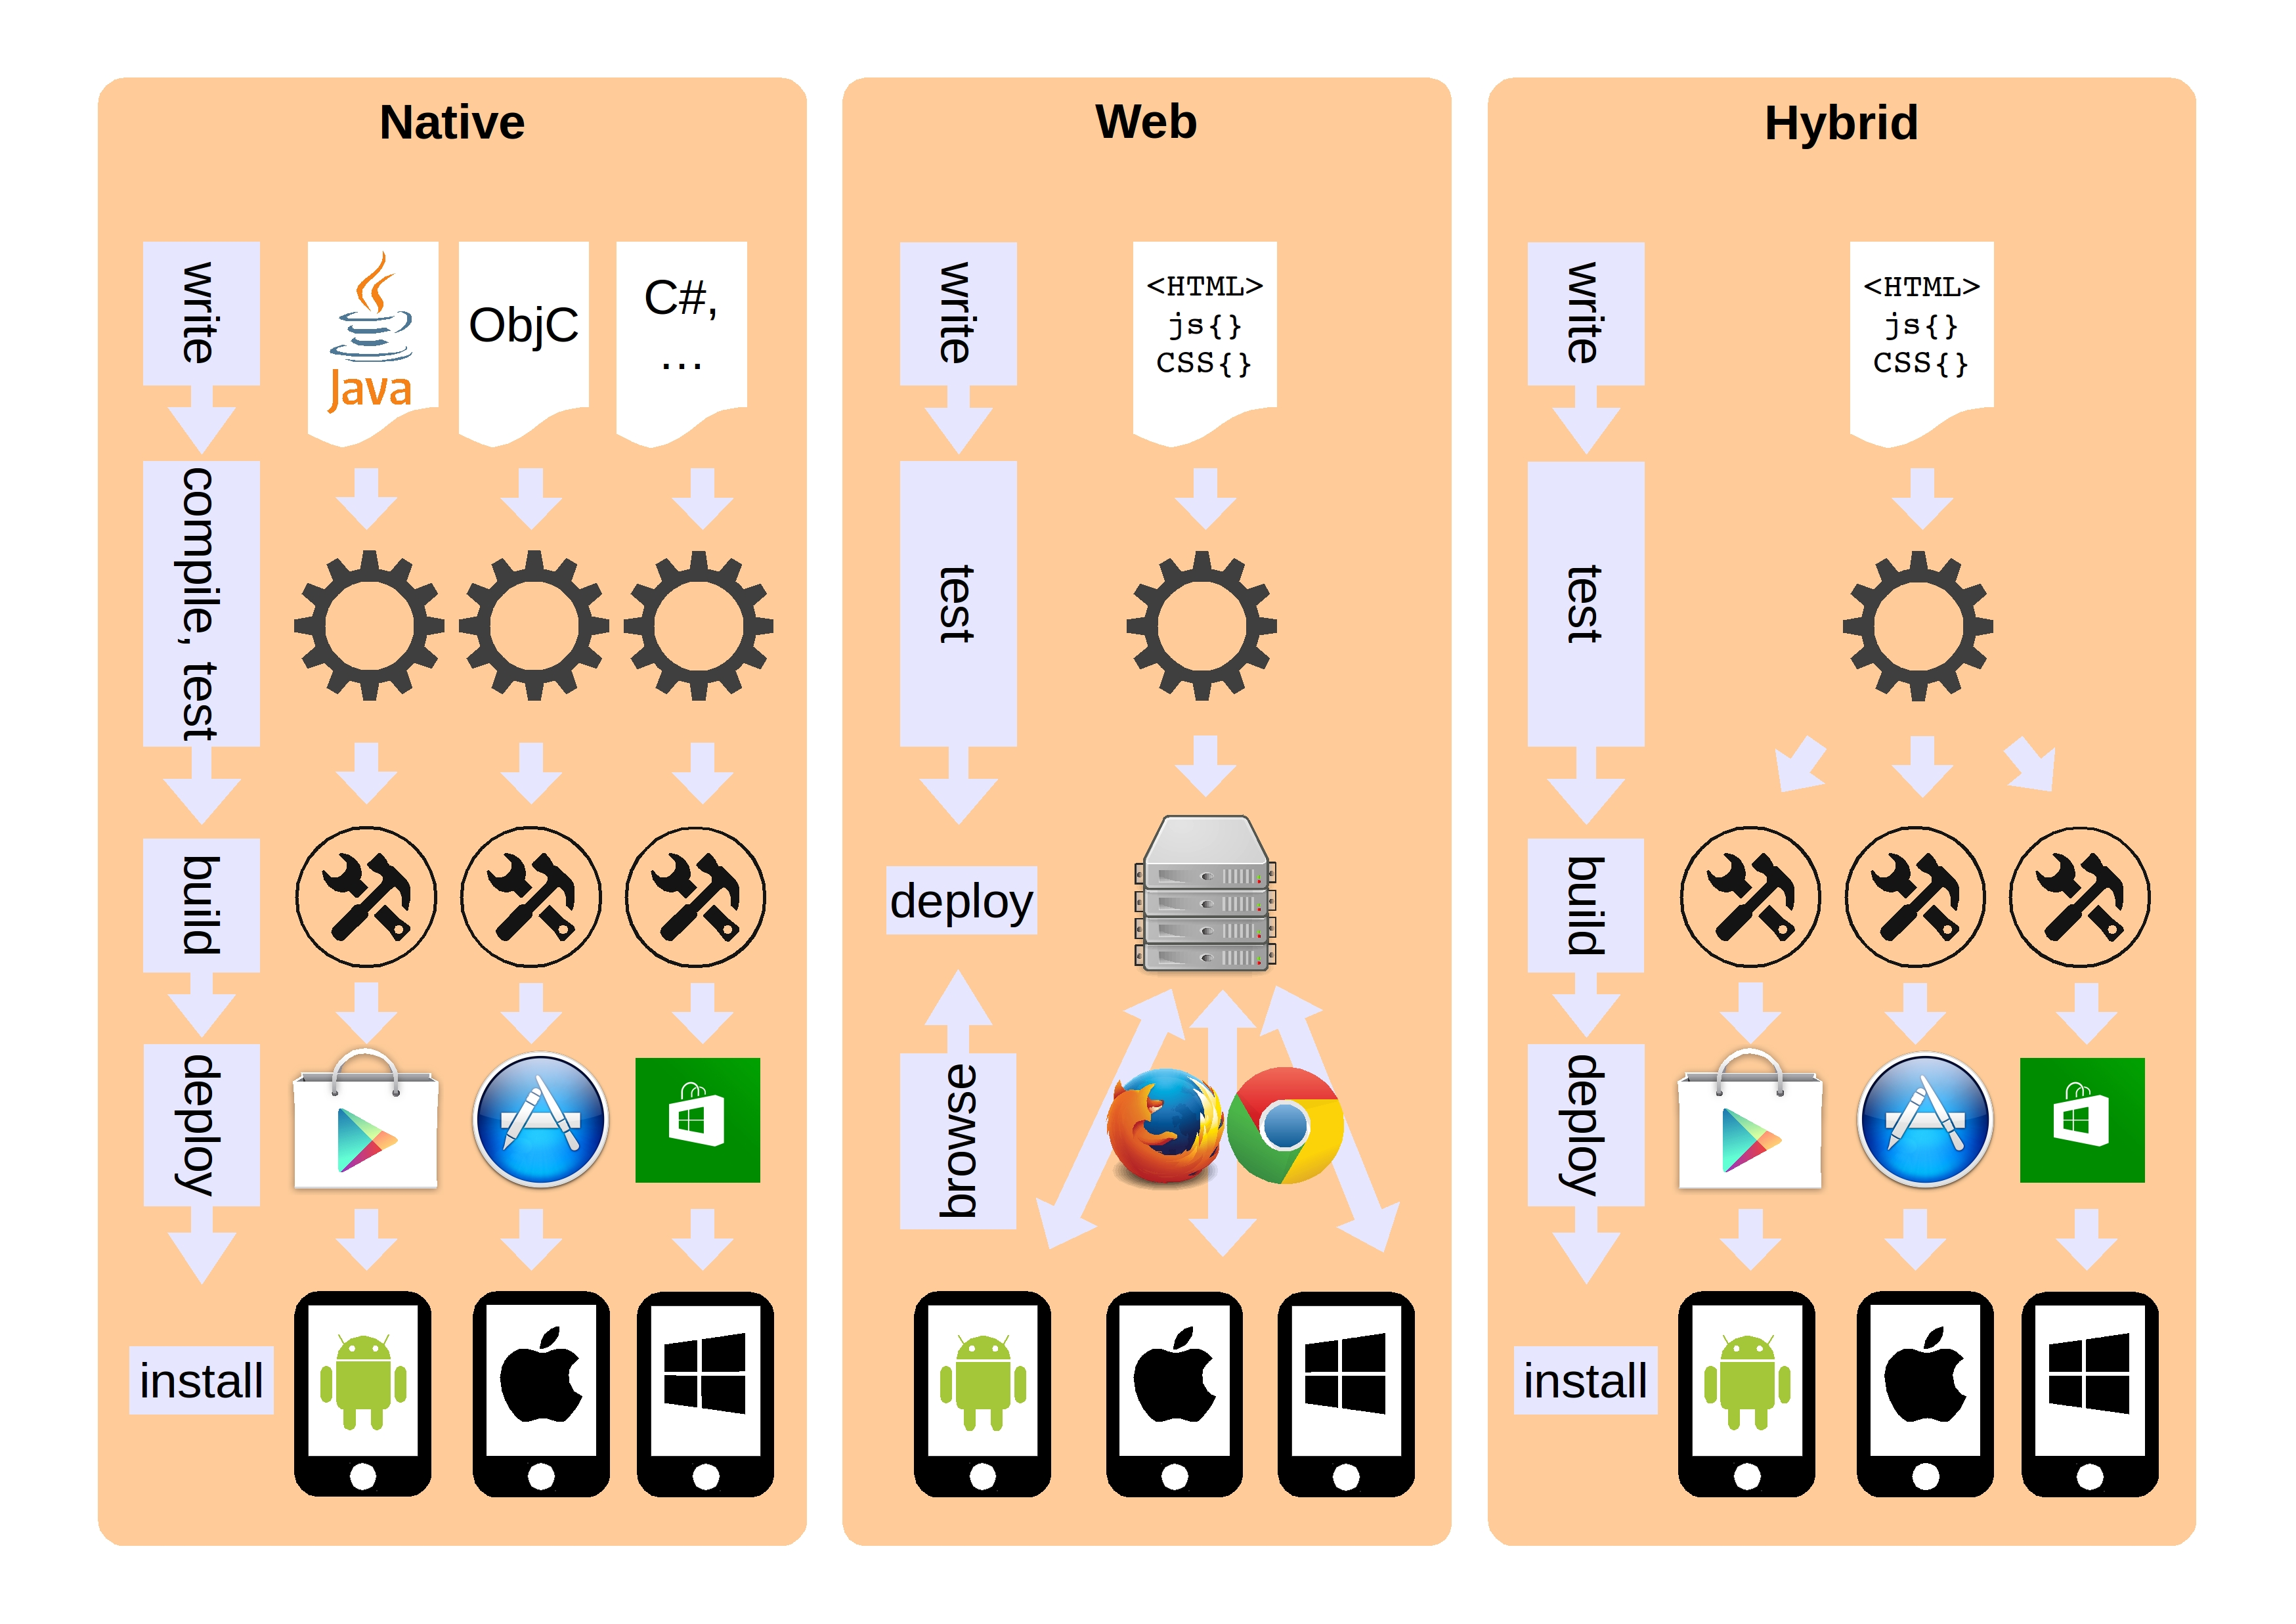
\includegraphics[width=1\linewidth]{./images/hybrid-apps-schaubild}
\caption[Schaubild Hybrid Apps]{Entwicklungsstufen der verschiedenen Arten von Apps. Während bei der nativen App der gesamte Entwicklungszyklus einmal pro Plattform durchlaufen werden muss, verringert sich der Aufwand für die Web-App erheblich. Bei der Hybrid-App muss die Anwendung zwar einmal für jede Plattform gebaut und ausgeliefert werden um die Schnittstellen für die nativen Plattformen zu implementieren, aber der hauptsächliche Entwicklungsaufwand des Programmierens und testens fällt aufgrund des generischen Charakters nur einmal an.}
\label{fig:hybrid-apps-schaubild}
\end{figure}

\section{Entwicklung von Hybriden Apps}\label{hybrid}

%TODO Hybride-App: Begriff erläutern

%TODO Vor-/Nachteile der hybriden App-Entwicklung

%TODO Plattformunabhängige App: Möglichkeiten?
%=========================================
	% Hybride App
	%------------
	%TODO Möglichkeiten zur hybriden App-entwicklung:
	%TODO - PhoneGap
	% - 

\begin{comment}
\subsection{Grundlegende Technologien}
Konkret heißt das, die Software wird als Webanwendung mit den zugehörigen Technologien (HTML, Javascript, CSS) entwickelt und für die jeweiligen benötigten Plattformen in eine native App eingebettet, welche hier allerdings hauptsächlich aus einer Web-View, also einer abgespeckten Variante eines Web-Browsers zur Anzeige der Webanwendung, besteht. Da dieser Ansatz der am häufigsten von Cross-Platform-Frameworks genutzte ist, \todo{nachweis!} stellt dieser auch den Schwerpunkt der in dieser Arbeit explorierten Technologien dar und soll hier näher erläutert werden. 

\subsection{Phonegap}
Die entscheidende Lücke auf dem Weg zur Hybrid-App zwischen Webanwendung und der nativen App schließt das Framework \emph{PhoneGap} von Adobe. 
Bei der Webanwendung taten sich in der Herleitung zwei grundlegende Problemfelder gegenüber der nativen App-Entwicklung auf. 
Zum Einen besteht eine Webanwendung aus mehreren Dokumenten, die auf einem Server liegen und nur über den Browser des Betriebssystems abgerufen werden, die Benutzung fühlt sich also für den Nutzer durch die ausbleibende Installation, die benötigte Internetverbindung und die optische Präsenz der Browser-Oberfläche nicht wie eine mobile App an. 
Zum Anderen können die Anforderungen an die Anwendung einen Zugriff auf native Features des Geräts oder seines Betriebssystems erfordern, der mittels herkömmlicher Webtechnologien nicht oder nur sehr eingeschränkt möglich sind. 

Für letzteres bietet PhoneGap eine Javascript-Bibliothek, die auf das Cross-Platform-Framework \emph{Cordova} von Apache aufbaut und den Zugriff auf native Features des jeweiligen Betriebssystems ermöglicht.\todo{wie genau, weiß ich noch nicht, noch rausfinden!}
Bei der konkreten Verwendung von nativen Features muss jedoch teilweise wieder auf die Unterstützung durch die jeweiligen Plattformen geachtet werden.\todo{oder zumindest muss deklariert werden, was verwendet werden soll. -> checken!}

Darüber hinaus übernimmt das Online-Portal \emph{PhoneGap~Build} den Bauprozess der App, also das Überführen in ein installierfähiges App-Format. 
Während der Entwickler ohne diesen Build-Service die verschiedenen Toolkits aller Zielplattformen lokal verwalten müsste, um Cordova zu verwenden,\{pg-doc-1} reicht es hier aus, die Web-Anwendung (beispielsweise per öffentlichem Git-Repository) auf das Portal hoch zu laden, den Build-Prozess im Browser abzuwarten und die fertigen Apps auf das gewünschten Zielgerät herunterzuladen und zu installieren. 

Für Auftraggeber oder Entwickler, die ihren Code als sehr sensibel und vertraulich ansehen, könnte diese Variante allerdings ein Problem darstellen sein, da der Quellcode dann stets auch auf den Servern von Adobe liegt.\todo{gehört vllt. eher woanders hin.}

\subsection{JQueryMobile}
Die Javascript-Bibliothek JQueryMobile baut auf JQuery auf und bietet ein Oberflächen-Toolkit für mobile Webseiten. Sie besteht zum Einen aus einer Javascript-Datei, die in die HTML-Seite eingebunden wird und zum Anderen aus einem CSS, das für das an mobile Touch-Geräte angepasste aussehen verantwortlich ist. 
So können einerseits UI-Elementen explizit Style-Klassen aus dem JQueryMobile-CSS zugewiesen werden, andererseits sorgt das JQuery-Javascript ohnehin bei allen verwendeten HTML-Elementen dafür, dass die Style-Klassen dynamisch vergeben werden und die UI-Komponenten somit ihr App-typisches Aussehen erhalten.
Lediglich mit dem zusätzlichen Attribut "data-role" werden den UI-Elementen Eigenschaftentypen zugewiesen, über die die JQueryMobile-Bibliothek erkennt, wie dieses dargestellt werden soll.
\marginpar{Konkreter, Beispiel?}

Dieser Mechanismus erleichtert es dem Frontend-Entwickler erheblich, eine auf Touchscreens ausgerichtete Oberfläche zu entwerfen, da er im Grunde neben einigen zusätzlichen Attributen sämtliche herkömmlichen HTML-Elemente verwenden kann. 

\subsection{KnockoutJS}
Auch bei \emph{Knockout} handelt es sich um eine Javascript-Bibliothek, die per \mbox{\texttt{<script>}-Tag} der HTML-Seite hinzugefügt wird. Knockout übernimmt mit einem MVVM (Model-View-ViewModel) das \emph{Data-Binding}, also die Verknüpfung zwischen Daten-Feldern im Programm und UI-Elementen.
So lässt sich die UI (View) sehr klar von der Programmlogik (Model) trennen, was der Lesbarkeit, Erweiterbarkeit und Wartbarkeit der Software zugute kommt.

Statt also Javascript mit HTML-String-Schnipseln zu vermischen, indem das DOM direkt manipuliert und UI-Elemente zur Laufzeit
\todo{gibt es bei javascript überhaupt eine laufzeit?} 
programmatisch erweitert werden, definiert der Entwickler in einem separaten Javascript ein View-Model und bindet mit dem HTML-Attribut \enquote{data-bind} \ eine bestimmte View-Eigenschaft an ein Datenfeld aus dem View-Model.
\marginpar{Konkreter, Beispiel, Grafik?}

\end{comment}
